\documentclass[10pt]{article}
\usepackage[margin=0.9in]{geometry}
\usepackage{amsmath,amssymb,booktabs,graphicx,microtype,caption}
\usepackage[hidelinks]{hyperref}
\graphicspath{{../figures/}{./}}
\captionsetup{font=small,labelfont=bf}
\newcommand{\Cov}{\operatorname{Cov}}
\newcommand{\Var}{\operatorname{Var}}
\newcommand{\bp}{\,\mathrm{bp}}

\title{\vspace{-1.2cm}Which Options Respond to Which Macro News,\\ and Do They Charge the Right Amount?}
\author{Michael Jafs\\[2pt] \small The Erd\H{o}s Institute, Introduction to Quantitative Methods in Finance, Fall 2026}
\date{November 2026}

\begin{document}
\maketitle
\vspace{-0.6cm}

\begin{abstract}
\noindent US macroeconomic data are released at 08:30 ET on dates known well in advance, meaning one-day options are forced to price each release the evening before. Using roughly 450 release mornings between May 2022 and October 2026, I measure how stocks respond to the interest-rate news contained in each release, how much extra options charge for it, and whether that charge was correct, with the last of these tested through a delta-hedged straddle. I find that the stock response per unit of bond response fell from $0.86$ in 2022--23 to $0.35$ in 2024--26 and now depends on the type of news. Options repriced accordingly, with the premium attached to the inflation release falling roughly fivefold. In 2022--23 options undercharged for release days relative to quiet days by $17\bp$ per trade ($t=-3.1$), whereas from 2024 onward this gap is consistent with zero. Finally, four results that initially appeared significant did not survive further testing, and I document each of them.
\end{abstract}

\section{Introduction and Motivation}
Several times a month the US government publishes a number capable of moving the entire market, with the consumer price index (CPI) and the jobs report being the most prominent examples. What makes these releases unusual as a source of risk is that, although nobody knows the value of the number, everybody knows exactly when it will arrive. Since an option expiring tomorrow is worth more if tomorrow is likely to be a large day, the price of a one-day option on the evening before a release contains the market's forecast of how much additional movement that release will cause.

This project asks whether that forecast was correct, and I approach the problem in three parts. I first measure how stocks actually respond to each type of release and whether that response has changed since 2022. I then measure the premium that options carry on the eve of each release, across release types, maturities and underlyings. Finally, I test whether that premium was right by selling the option, hedging it using the methods developed in the course, and comparing the outcome on release evenings with the outcome on ordinary evenings. For the inflation release an additional and fully independent source of information exists. Kalshi, a regulated prediction market, lists contracts on the value of the CPI print itself, which provides a direct measurement of how uncertain the market is about the number. As I show in Section~\ref{sec:kalshi}, this allows the option premium to be separated into the size of the news and the sensitivity of stocks to it.

\section{Data}
Release dates for CPI, the Employment Situation (hereafter ``jobs''), PCE, GDP, retail sales, PPI and jobless claims are taken from the FRED release calendar, with FOMC meeting dates added by hand. Since several releases can fall on the same day, I label each day by its highest-ranked event in the order CPI, jobs, FOMC, PCE, GDP, retail sales, PPI and claims. A day containing none of these is referred to as a \emph{quiet day}, and quiet days serve as the benchmark throughout. In total the sample contains 452 release days and 661 quiet days. For prices I use one-minute bars for SPY, TLT, QQQ and IWM including the pre-market session, the Cboe VIX1D, VIX9D and VIX indices, and, from February 2024 onward, the last traded prices of next-day at-the-money options on SPY, QQQ and IWM. The Kalshi data consist of core CPI contract ladders for 52 releases. I also note that the split between the two periods at 1 January 2024 was fixed before any of the data were examined.

\section{Formalism}
\subsection{Stock Response to Rate News}
A release affects stocks largely through interest rates, since news that makes higher rates more likely pushes bond prices down within seconds. Whether stocks follow depends on how the news is interpreted. Let $r$ and $b$ denote the SPY and TLT returns between 08:30 and 08:45. On any given morning both returns contain background shocks $(u_r,u_b)$, while on a release morning the news contributes an additional shock $n$ to bonds to which stocks respond proportionally, such that
\begin{equation}
b = n + u_b, \qquad r = \gamma\, n + u_r .
\end{equation}
If the background shocks follow the same distribution on release and quiet mornings and are independent of $n$, then the difference in covariances between the two types of morning is $\gamma\Var(n)$ and the difference in bond variances is $\Var(n)$. Taking the ratio gives
\begin{equation}
\gamma \;=\; \frac{\Cov_{\mathrm{rel}}(r,b)-\Cov_{\mathrm{quiet}}(r,b)}{\Var_{\mathrm{rel}}(b)-\Var_{\mathrm{quiet}}(b)} ,
\label{eq:gamma}
\end{equation}
which is the identification-through-heteroskedasticity estimator of Rigobon and Sack (2004). One can think of $\gamma$ as the percent move in stocks per one percent move in bonds that is caused by the news. A value near one indicates that the news is being read as tighter monetary policy, whereas a value near zero indicates that bonds move while stocks do not. The advantage of this approach is that it requires no measurement of the surprise itself and can therefore be applied to every release. The obvious alternative, a regression of $r$ on $b$, would instead be biased toward the everyday relationship between stocks and bonds. Confidence intervals are obtained from a percentile bootstrap in which release days and quiet days are resampled separately, and I withhold an estimate whenever the bond variance on release mornings is less than $1.5$ times its value on quiet mornings.

\subsection{What Options Charge}
The one-day implied variance is given by $V_t=\mathrm{VIX1D}_t^2/252$, expressed in units of $\%^2$. I define the \emph{event premium} for a release on day $t$ as the implied variance on the preceding evening relative to its level on nearby quiet evenings,
\begin{equation}
\pi_t \;=\; V_{t-1} - \operatorname{median}\bigl\{V_s \;\big|\; s \text{ a quiet eve},\ |s-(t-1)|\le 5\bigr\}.
\end{equation}
From February 2024 the same quantity is computed from traded prices, where $V$ is obtained by inverting the Black--Scholes price of the at-the-money straddle.

\subsection{Testing Whether the Charge Was Right}
To test the premium I rely on the delta-hedging framework from the course. On each evening a one-day at-the-money straddle is sold at the implied volatility $\sigma_{\mathrm{imp}}$ and hedged by holding the Black--Scholes delta in the underlying. Since no rebalancing is possible overnight, the position is held through the gap, rebalanced at the open, and settled at the close at $|S_T-K|$. To second order the profit of the seller is
\begin{equation}
\text{P\&L} \;\approx\; \sum_i \tfrac12\,\Gamma_i S_i^2\bigl(\sigma_{\mathrm{imp}}^2-\sigma_{\mathrm{real},i}^2\bigr)\Delta t ,
\end{equation}
meaning the seller profits whenever implied variance exceeds realized variance. I report this profit in basis points of the spot price. The quantity of interest is then the mean profit on release evenings minus the mean profit on quiet evenings within the same period, which has the benefit of removing any bias common to all days. Before applying the hedging engine to real prices, I verified it on simulated geometric Brownian motion, where the mean profit must equal the Black--Scholes price at the implied variance minus the price at the true variance. The engine reproduces this to within Monte Carlo error (for example, $-17.0\bp$ compared with $-16.9\bp$ when realized variance is $1.5$ times implied).

\subsection{The Kalshi Decomposition for CPI}
\label{sec:kalshi}
A Kalshi contract paying out if CPI exceeds a strike $k$ is priced at the probability of that outcome. The ladder of strikes therefore traces out the distribution of the print, from which I compute a mean $\mu_K$ and a standard deviation $\sigma_K$. Defining the surprise as $s=x-\mu_K$, where $x$ is the published value, and modelling the stock reaction as $r=\beta s+\varepsilon$, the variance attributable to the surprise is $\beta^2\sigma_K^2$. The sensitivity that option prices implicitly assume is then
\begin{equation}
|\beta_{\mathrm{impl}}| \;=\; \sqrt{\bar\pi\,/\,\overline{\sigma_K^2}} ,
\end{equation}
which can be compared directly with the regression estimate $\hat\beta$. Since $\beta$ need not be constant in time, I additionally estimate the state-space model $\beta_t=\beta_{t-1}+w_t$, $r_t=\beta_t s_t+e_t$ using a Kalman filter with parameters fit by maximum likelihood. In this case the fair premium for release $t$ is computed from the one-step-ahead prediction alone, $(m_{t|t-1}^2+P_{t|t-1})\,\sigma_{K,t}^2$, so that no future information enters. I also note that the closest related work is that of Knox, Londono, Samadi and Vissing-Jorgensen (2025), who use daily S\&P 500 option expirations to identify the days carrying an elevated equity premium and who decompose that premium into the variance of the news and the sensitivity of stocks to it. The approach taken here differs in that the variance of the news is read directly from a prediction market the evening before, and in that I study the variance priced by options as opposed to the equity premium.

\section{Results}
\begin{figure}[h]
\centering
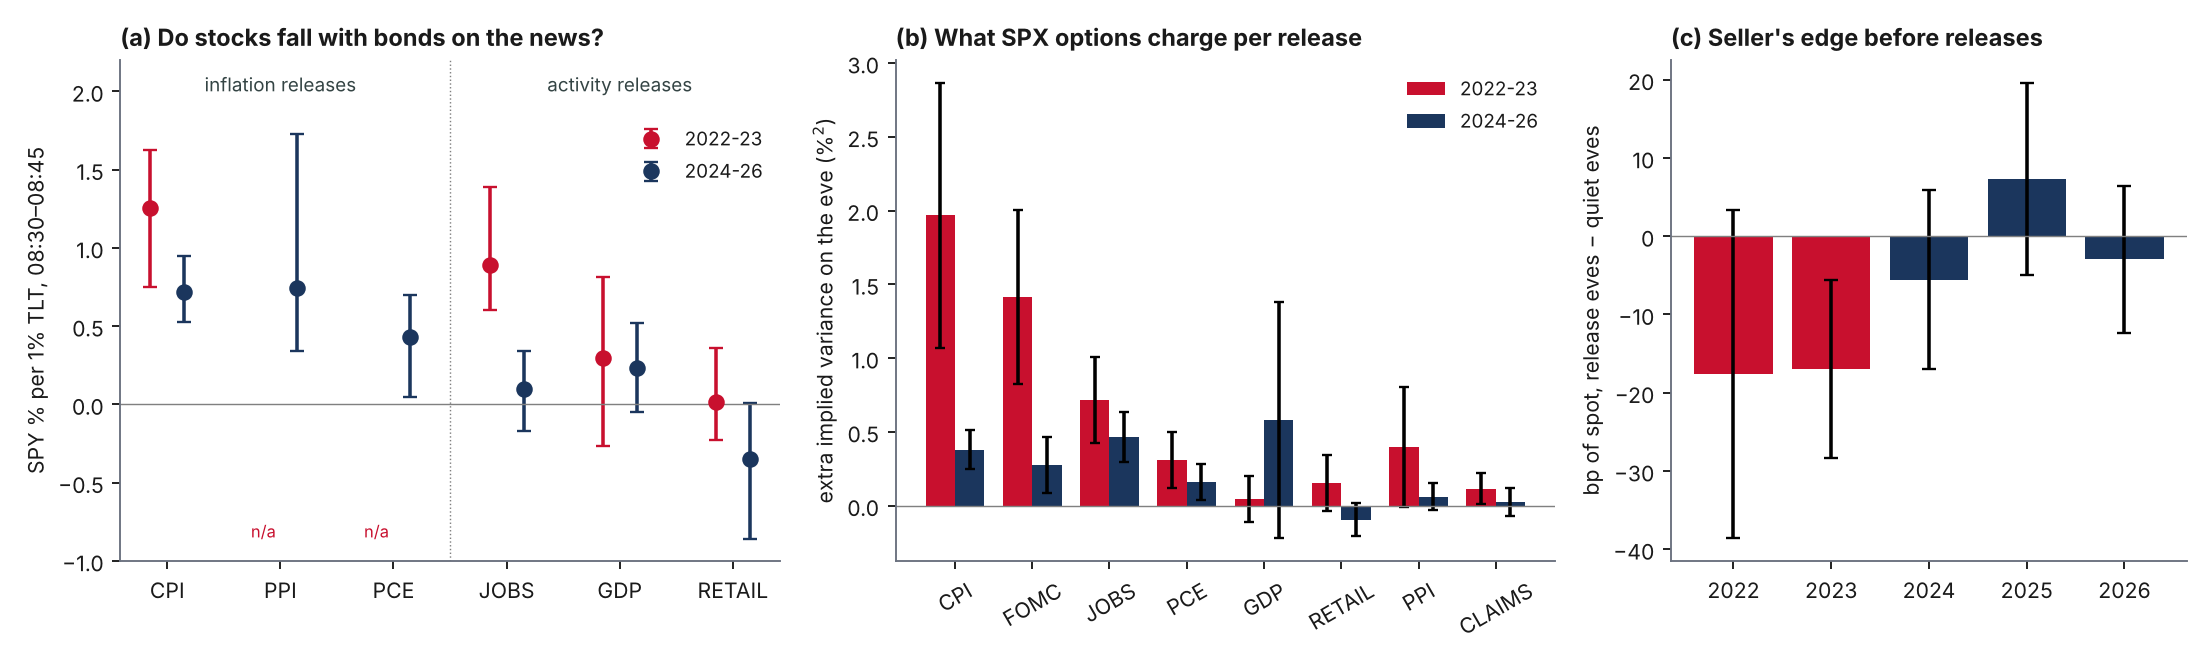
\includegraphics[width=\textwidth]{summary.png}
\caption{(a) The stock response $\gamma$ by release type and period with 95\% bootstrap intervals. (b) The event premium in one-day SPX implied variance. (c) The seller's profit on release evenings minus quiet evenings, by year.}
\label{fig:summary}
\end{figure}

\subsection{The Stock Response Has More Than Halved and Now Depends on the News}
Pooling all releases except jobless claims, $\gamma$ fell from $0.86$ $[0.53,1.14]$ in 2022--23 to $0.35$ $[0.17,0.52]$ in 2024--26, a difference of $0.52$ $[0.15,0.85]$. Estimated year by year the values are $1.16$, $0.43$, $0.37$, $0.35$ and $0.27$, which places the break between 2022 and 2023. More interesting is how this decline is distributed across release types, as shown in panel (a) of Figure~\ref{fig:summary}. In 2024--26 the inflation releases (CPI, PPI and PCE) retain $\gamma=0.66$, whereas the activity releases (jobs, GDP and retail sales) sit at $0.05$, with the difference between the two groups lying in $[0.36,0.89]$. The jobs report provides the cleanest example. Bonds react to it as strongly as before, yet stocks no longer follow, and $\gamma$ has fallen from $0.89$ to $0.10$. A natural interpretation is that a strong jobs number in 2022 meant that the Fed would raise rates, whereas it now also signals a healthy economy.

\begin{table}[h]
\centering\small
\begin{tabular}{lcccc}
\toprule
 & \multicolumn{2}{c}{$\gamma$ (SPY \% per 1\% TLT)} & \multicolumn{2}{c}{Event premium $\pi$ (\%$^2$)}\\
\cmidrule(lr){2-3}\cmidrule(lr){4-5}
Release & 2022--23 & 2024--26 & 2022--23 & 2024--26\\
\midrule
CPI  & $1.25\ [0.75,1.62]$ & $0.71\ [0.53,0.95]$ & $1.97\ (t=4.3)$ & $0.38\ (t=5.6)$\\
Jobs & $0.89\ [0.60,1.39]$ & $0.10\ [-0.17,0.34]$ & $0.71\ (t=4.8)$ & $0.46\ (t=5.3)$\\
FOMC & n/a & n/a & $1.41\ (t=4.7)$ & $0.27\ (t=2.8)$\\
PCE  & not identified & $0.43\ [0.05,0.70]$ & $0.31\ (t=3.2)$ & $0.16\ (t=2.6)$\\
\bottomrule
\end{tabular}
\caption{The stock response and option premium for the four releases that options price. GDP, retail sales, PPI and jobless claims carry no significant premium.}
\label{tab:main}
\end{table}

\subsection{Options Price Four Releases and Repriced Them}
Only four releases carry a significant premium in one-day implied variance, namely CPI, FOMC, jobs and PCE (Table~\ref{tab:main}). The CPI premium fell roughly fivefold between the two periods while the jobs premium fell by only a third, such that CPI went from costing nearly three times as much as the jobs report to costing about the same. The premium is also visible further along the volatility curve. When CPI passed in 2022--23, one-day, nine-day and thirty-day options lost $1.5$, $2.4$ and $2.7\,\%^2$ of total implied variance relative to quiet days.

\subsection{Options Undercharged for Release Days in 2022--23}
Priced at VIX1D, the seller of the hedged straddle earned $-3.2\bp$ across 174 release evenings compared with $+14.1\bp$ across 235 quiet evenings, a difference of $-17.3\bp$ ($t=-3.1$). The origin of this gap is that realized variance amounted to $95\%$ of implied variance on release days but only $77\%$ on quiet days. In 2024--26 the same difference is $-0.6\bp$ ($t=-0.2$, from 278 and 426 evenings respectively). I therefore conclude that the market underpriced scheduled news during the inflation shock and had corrected for this by 2024.

\subsection{No Ordinary-Day Premium at Traded Prices}
Although VIX1D is widely quoted, it is an index and not a price at which one can trade. Using traded option prices I find that at-the-money volatility is $0.94$ of VIX1D. As a consequence, the apparent quiet-evening profit of $7.8\bp$ obtained at VIX1D becomes $3.3$, $1.6$ and $4.1\bp$ for SPY, QQQ and IWM respectively, none of which is significant and all of which are before bid--ask costs. The traded prices additionally allow a comparison across underlyings. Relative to its own quiet-day variance, IWM prices CPI, jobs and FOMC roughly twice as heavily as SPY does, which is consistent with small companies being more exposed to interest rates.

\subsection{Kalshi Confirms the Pricing of CPI}
In 2022--23 the sensitivity implied by options and Kalshi together is $|\beta_{\mathrm{impl}}|=9.3$ $[6.9,11.6]$, in close agreement with the realized $\hat\beta=-9.8$ percent per percentage point of surprise. In 2024--26 the reaction measured in the 15-minute window is $-3.8$ ($t=-3.4$), and the excess premium from the Kalman filter is $-0.02\,\%^2$ ($t=-0.3$), meaning option prices remain consistent with the lower sensitivity. As a further check, estimating $\gamma$ with the Kalshi surprise as an instrument gives $1.47\to0.75$, compared with $1.25\to0.71$ from Equation~\ref{eq:gamma}, which uses no Kalshi data at all. I also find that although the Kalshi mean is unbiased, its distribution is roughly $1.25$ times too wide.

\section{Results That Did Not Survive Testing}
Over the course of the project, four findings appeared convincing and were later withdrawn. I include them here since the tests that removed them are as much a part of the work as the results that remain.

The first was that options overprice the sensitivity of stocks to CPI by a factor of two to three in 2024--26. A static comparison gave $|\beta_{\mathrm{impl}}|=5.6$ against $\hat\beta\approx-2$. However, once $\beta_t$ is allowed to vary in time the excess vanishes, and when each release is moved to a placebo day three to ten sessions away the same estimator returns a value of roughly $3$ from noise alone. The second was that the stock reaction to CPI had disappeared after 2023. This turned out to hold only for overnight returns ($t=-1.0$), where unrelated noise of $0.8\%$ hides a signal of $0.3\%$. In the 15 minutes following the release the surprise explains $37\%$ of the variance. The third was that selling one-day options earns a steady premium, which is an artifact of pricing at VIX1D as described above. The fourth was that sellers of IWM options earn $58\bp$ before FOMC meetings ($t=3.6$). Here a dividend filter had removed 9 of the 21 meetings, and with all 21 included the figure is $35\bp$ ($t=1.2$).

I also performed an injection--recovery test on simulated panels, which shows that the Kalshi design has only about $30\%$ power against a mispricing of the size described in the first case. The CPI result for 2024--26 should therefore be read as an absence of evidence for mispricing and not as proof that none exists. Moreover, neither using the unrounded CPI print nor adding the headline surprise changed $R^2$ by more than $0.04$.

\section{Limitations}
The sample covers four and a half years and contains a single change of regime, so I cannot say how general the pattern is. VIX1D is backfilled by Cboe before April 2023 and traded option prices only begin in February 2024, meaning the underpricing found in 2022--23 rests on an index, although it also holds in the portion of 2023 where VIX1D was live ($-13.5\bp$, $t=-2.3$). The traded prices I use are last trades and do not include bid--ask costs. Furthermore, since many combinations of release and underlying were examined, I only claim the pooled results. Finally, the week of 3--11 April 2025 is excluded from the option tables, and this choice was made after seeing its effect.

\section{Concluding Remarks}
In 2022, news that raised interest rates lowered stocks regardless of its source. Since 2023 this remains true for inflation news at roughly half the strength, and is no longer true for news about economic activity. Option markets priced four releases as events and repriced them as the regime changed. They charged too little for release days while the change was under way and have priced them fairly since 2024. Although I find no tradeable edge in the recent data, the contribution of this work lies in the measurement itself and in the tests that separate it from artifacts. As next steps I would obtain historical option quotes for 2022--23 to confirm the underpricing at traded prices, include bid--ask costs, and extend the prediction-market check to the jobs report as Kalshi's history grows.

\medskip\noindent The code, a results notebook and all derived data are available at \url{https://github.com/mikejafs/macro_news_options_project}.

\begin{thebibliography}{9}\small
\bibitem{rs} R.~Rigobon and B.~Sack (2004). The impact of monetary policy on asset prices. \emph{Journal of Monetary Economics} 51(8).
\bibitem{bk} G.~Bakshi and N.~Kapadia (2003). Delta-hedged gains and the negative market volatility risk premium. \emph{Review of Financial Studies} 16(2).
\bibitem{klsv} B.~Knox, J.~M.~Londono, M.~Samadi and A.~Vissing-Jorgensen (2025). Equity premium events. Working paper, Federal Reserve Board.
\end{thebibliography}
\end{document}
